\section{Density Transformation}

\mode<presentation>{
\begin{frame} 
    \begin{center} \huge
        \secname
    \end{center}
    
    \begin{center}
    Sampling from your favorite distribution.
    \end{center}
    
    \pause
    
\slidesonly{
\begin{center}
	
\includegraphics[width=0.3\textwidth]{img/meme_wheresica}
\end{center}
}
\end{frame}
}

\begin{frame}{\secname}

\notesonly{

\underline{Outline:}

Before we tackle ICA itself, we first look at the more basic principle of \emph{density transformation} and 
the \emph{conservation of probability}.\\
We start with more specific cases of applying density transformations, 
namely \emph{pseudo random number generators} (PRNG) and what the inverse of \emph{cumulative distribution functions (cdf)} can be used for.\\
Finally we discuss how to generalize this in order to transform one probability density function (pdf) into another.
}

\slidesonly{
First we need to cover the basic principle of \emph{density transformation} and 
the \emph{conservation of probability}. We start with specific cases:

\begin{enumerate}
\item pseudo random number generators
\item what is the inverse of \emph{cumulative distribution functions (cdf)} good for?
\end{enumerate}

\pause 

Then generalize this to transform one probability density function (pdf) into another. We will make direct use of density transformation in \emph{Infomax ICA}.

\pause

\slidesonly{
\begin{center}
	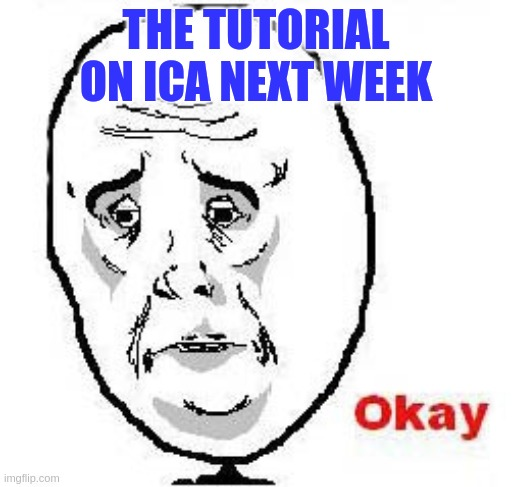
\includegraphics[width=0.3\textwidth]{img/meme_icanextweek}
\end{center}
}

}

\end{frame}

\subsection{PRNG}

\mode<presentation>{

\begin{frame}\frametitle{Random Number Generators}

\pause

\slidesonly{
\begin{center}
	
\includegraphics[width=0.3\textwidth]{img/meme_onlypseudo}
\end{center}
}

\end{frame}

}

\begin{frame}\frametitle{\textbf{Pseudo} Random Number Generators (\subsecname)}

\question{How can we sample from the uniform distribution $\in \lbrack0, 1)$?}

\begin{itemize}
\item create a sequence, preferably an aperiodic one,
\item maintain a minimal pattern, also no sub-sequences,
\item keep elements in the range of $\lbrack0, 1)$
\end{itemize}

\pause

\svspace{5mm}

Pseudo-random is essentially deterministic, but determinism has its advantages:
\begin{enumerate}
	\item \emph{reproducible} sequences
	\item efficiency; the starting element or ``seed'' and length of the sequence is sufficient to represent the entire sequence.
\end{enumerate}

\end{frame}

\subsubsection{Linear congruential generator (LCG)}

\begin{frame}{\subsubsecname}

LCG is a method for generating pseudo random samples from the uniform distribution.

Start with a seed $y_0 \in \overbrace{\left\{0,\ldots,m-1\right\}}^{=:\;\mathcal{M}}$ with $m \in \N$ ($m$ controls the granularity). 
The next sample $y_t$ is computed as:

\begin{equation}
y_t = \left( \, a \; y_{t-1} \; + \; b \, \right) \, \text{mod} \; m,
\end{equation}
where\\[-0.7cm]
\begin{align*}
a \in \mathcal{M}&\; \text{is the multiplier,} \\
b \in \mathcal{M}&\; \text{is the increment.}
\end{align*}

Then $u_t = \frac{y_t}{m} \approx \,\mathcal{U} \in \lbrack0, 1)$.

\pause

\slidesonly{
\vspace{5mm}
Let's see the LCG in action.
}

\end{frame}

\begin{frame}

Although finicky and requiring careful parametrization, LCG gives us something for drawing from a uniform distribution. 
\svspace{5mm}
Next, we look at how to draw samples of a random variable $X$ with a desired pdf $p_X(x)$. 
using uniformly sampled values $\tilde z \in [0,1]$.

\end{frame}

